\documentclass[
  article,
  12pt,
  oneside,
  a4paper,
  english,
  brazil,
  chapter=TITLE,
  section=TITLE,
  subsection=TITLE
]{abntex2}

\usepackage[T1]{fontenc}
\usepackage[utf8]{inputenc}
\usepackage{newtxtext,newtxmath}
\usepackage{indentfirst}
\usepackage{graphicx}
\usepackage{microtype}
\usepackage{placeins}
\usepackage{listingsutf8}

\lstset{
  inputencoding=utf8/latin1,
  language=Python,
  basicstyle=\ttfamily\footnotesize,
  breaklines=true,
  columns=fullflexible,
  keepspaces=true,
  showstringspaces=false,
  tabsize=2,
  frame=single,
  numbers=left,
  numberstyle=\tiny,
  numbersep=8pt,
  xleftmargin=2em,
  framexleftmargin=1.6em,
  aboveskip=8pt,
  belowskip=8pt
}

\makeatletter
\g@addto@macro{\UrlBreaks}{\do\_}
\makeatother

\titulo{Impacto das redes sociais na saúde mental de estudantes}
\autor{Ian de Araújo \and Jardson Alan}
\local{Rio Grande do Norte}
\data{2026}
\instituicao{%
  Instituto Federal de Educação, Ciência e Tecnologia\\
  do Rio Grande do Norte%
}
\preambulo{%
  Artigo apresentado à disciplina de Análise de Dados do Instituto Federal
  de Educação, Ciência e Tecnologia do Rio Grande do Norte, com o registro
  do conjunto de dados e do pré-processamento do projeto.%
}

\hypersetup{
  hidelinks,
  pdftitle={Impacto das redes sociais na saúde mental de estudantes},
  pdfauthor={Ian de Araújo; Jardson Alan}
}

\renewcommand{\imprimircapa}{%
  \begin{capa}%
    \SingleSpacing
    \begin{center}
      \imprimirinstituicao\par
      \vspace*{\fill}
      \imprimirautor\par
      \vspace*{\fill}
      {\bfseries\imprimirtitulo\par}
      \vspace*{\fill}
      \imprimirlocal\par
      \imprimirdata\par
    \end{center}
    \vspace*{1cm}
  \end{capa}%
}

\renewcommand{\folhaderostocontent}{%
  \SingleSpacing
  \begin{center}
    \imprimirautor\par
  \end{center}
  \vspace{3.2cm}
  \begin{center}
    {\bfseries\imprimirtitulo\par}
  \end{center}
  \vspace{2.2cm}
  \hfill
  \begin{minipage}[t]{.46\textwidth}
    \imprimirpreambulo
  \end{minipage}
  \vspace{3.2cm}
  \begin{center}
    \imprimirlocal\par
    \imprimirdata\par
  \end{center}
}

\AtBeginDocument{%
  \setlength{\absleftindent}{0pt}%
  \setlength{\absrightindent}{0pt}%
  \setlength{\absparindent}{0pt}%
  \setlength{\emergencystretch}{2.5em}%
}

\graphicspath{{../figures/}}

\begin{document}

\pretextual
\imprimircapa
\imprimirfolhaderosto

\textual

\begin{center}
  \bfseries\imprimirtitulo
\end{center}

\vspace{0.75\baselineskip}
\noindent Ian de Araújo\footnotemark{} e Jardson Alan\footnotemark[\value{footnote}]
\footnotetext{Estudantes da disciplina de Análise de Dados do Instituto Federal de Educação, Ciência e Tecnologia do Rio Grande do Norte.}

\begin{resumo}
Este estudo analisa dados de 4.500 estudantes, do ensino médio à pós-graduação, para investigar se o maior tempo diário de uso de redes sociais está associado a um menor índice de saúde mental. Busca-se medir a intensidade dessa relação e verificar se ela se mantém ao considerar idade, gênero e nível acadêmico. O atributo alvo é o \texttt{Mental\_Health\_Index}. O principal atributo explicativo é o \texttt{Daily\_Usage\_Hours}. O arquivo reúne 16 atributos demográficos, comportamentais e psicométricos, obtidos do conjunto \textit{Impact of Social Media on Life}. Não há valores ausentes no alvo nem nas horas diárias. Há 46 registros ausentes em \texttt{Perceived\_Stress\_Score} e 85 em \texttt{Academic\_Performance\_GPA}. O pré-processamento mantém as 4.500 linhas, seleciona as colunas numéricas e preenche cada vazio de estresse e de GPA com a média truncada de 10\% em cada extremidade, calculada entre os estudantes da mesma idade. Em seguida, cada coluna numérica passa a ter média 0 e desvio-padrão 1. A comparação entre idade e índice conserva o desenho da nuvem, e os eixos passam a estar em desvios-padrão.

\vspace{\onelineskip}
\noindent
\textbf{Palavras-chave}: Saúde mental. Redes sociais. Pré-processamento. Média truncada. \mbox{Padronização.}
\end{resumo}

\section{Objetivo}

Este estudo pretende analisar dados de 4.500 estudantes, do ensino médio à pós-graduação, para investigar se o maior tempo diário de uso de redes sociais está associado a um menor índice de saúde mental. Busca-se medir a intensidade dessa relação e verificar se ela se mantém ao considerar fatores como idade, gênero e nível acadêmico.

O atributo alvo é o \texttt{Mental\_Health\_Index} (índice de saúde mental). Ele será analisado em função do tempo diário de uso de redes sociais (\texttt{Daily\_Usage\_Hours}), que é o principal atributo explicativo. Idade (\texttt{Age}), gênero (\texttt{Gender}) e nível acadêmico (\texttt{Academic\_Level}) entram como fatores de controle.

\section{Conjunto de dados}

O arquivo \texttt{data/raw/}\allowbreak\texttt{dataset.csv} reúne respostas de 4.500 estudantes, do ensino médio à pós-graduação, sobre tempo de tela, sono, estresse e desempenho acadêmico. São 16 atributos demográficos, comportamentais e psicométricos. A fonte é o conjunto \textit{Impact of Social Media on Life}, publicado por Yadav (2026) no Kaggle sob licença CC0 (domínio público). No Kaggle, o nome do arquivo é \texttt{Social\_media\_impact\_on\_life.csv}.

No arquivo local não há valores ausentes em \texttt{Mental\_Health\_Index} nem em \texttt{Daily\_Usage\_Hours}. Há ausências em \texttt{Perceived\_Stress\_Score} (46 registros) e em \texttt{Academic\_Performance\_GPA} (85 registros).

\subsection{Atributos}

A Tabela~\ref{tab:atributos} apresenta os 16 atributos do arquivo, com o tipo e a descrição de cada um.

\begin{table}[htb]
  \centering
  \caption{Atributos do conjunto de dados}
  \label{tab:atributos}
  \small
  \begin{tabular}{llp{7.2cm}}
    \toprule
    Atributo & Tipo & Descrição \\
    \midrule
    \texttt{Student\_ID} & Texto & Identificador único do estudante \\
    \texttt{Age} & Inteiro & Idade em anos completos (15 a 26) \\
    \texttt{Gender} & Categórico & Female, Male, Non-Binary ou Prefer not to say \\
    \texttt{Academic\_Level} & Categórico & High School, Undergraduate ou Postgraduate \\
    \texttt{Primary\_Platform} & Categórico & Instagram, TikTok, YouTube, Snapchat, X (Twitter), Reddit ou LinkedIn \\
    \texttt{Daily\_Usage\_Hours} & Numérico & Tempo médio diário em redes sociais, em horas. Atributo explicativo principal \\
    \texttt{Weekend\_Extra\_Hours} & Numérico & Horas extras de tela nos fins de semana \\
    \texttt{Device\_Type} & Categórico & Smartphone, Laptop/PC ou Tablet \\
    \texttt{Sleep\_Duration\_Hours} & Numérico & Duração média do sono por noite, em horas \\
    \texttt{Sleep\_Quality\_Score} & Inteiro & Qualidade do sono, de 1 (muito ruim) a 5 (excelente) \\
    \texttt{Late\_Night\_Usage} & Booleano & Uso frequente de tela depois da meia-noite \\
    \texttt{Social\_Comparison\_Frequency} & Categórico & Never, Rarely, Sometimes, Frequently ou Always \\
    \texttt{Perceived\_Stress\_Score} & Numérico & Estresse percebido na escala PSS, de 0 a 40 \\
    \texttt{Mental\_Health\_Index} & Inteiro & Índice de bem-estar, de 32 a 98. Atributo alvo \\
    \texttt{Academic\_Performance\_GPA} & Numérico & GPA acumulado, de 1,9 a 4,0 \\
    \texttt{Overall\_Impact} & Categórico & Beneficial, Neutral ou Negative \\
    \bottomrule
  \end{tabular}
  \fonte{Elaborado pelos autores (2026).}
\end{table}

\section{Pré-processamento}

O registro desta etapa é de 23 de outubro de 2026. O fluxo é o \texttt{main.py}, sobre \texttt{data/raw/}\allowbreak\texttt{dataset.csv}.

A leitura fica em \texttt{src/data/}\allowbreak\texttt{load\_data.py} e devolve a tabela inteira. As 4.500 linhas permanecem, porque a ausência está em células de duas colunas: 46 registros em \texttt{Perceived\_Stress\_Score} e 85 em \texttt{Academic\_Performance\_GPA}. \texttt{Mental\_Health\_Index} e \texttt{Daily\_Usage\_Hours} seguem com os valores observados.

A seleção numérica está em \texttt{src/preprocessing/}\allowbreak\texttt{clean\_data.py} e mantém as colunas a seguir. \texttt{Student\_ID} e os atributos categóricos ou booleanos ficam fora desta etapa. Média e padronização se aplicam às medidas numéricas. \texttt{Age} permanece na tabela e define o grupo do preenchimento.

\begin{itemize}[topsep=4pt,itemsep=1pt,parsep=0pt]
  \item \texttt{Age} e \texttt{Daily\_Usage\_Hours}.
  \item \texttt{Weekend\_Extra\_Hours} e \texttt{Sleep\_Duration\_Hours}.
  \item \texttt{Sleep\_Quality\_Score} e \texttt{Perceived\_Stress\_Score}.
  \item \texttt{Mental\_Health\_Index} e \texttt{Academic\_Performance\_GPA}.
\end{itemize}

Cada vazio de estresse e de GPA recebe a média truncada de 10\% em cada extremidade, calculada em \texttt{src/calculations/}\allowbreak\texttt{descriptive\_statistics.py} entre os estudantes da mesma idade. O preenchimento grava esse valor só na célula vazia.

As colunas numéricas estão em escalas diferentes: idade de 15 a 26 anos, horas de uso, de sono e de fim de semana, qualidade do sono de 1 a 5, estresse de 0 a 40, índice de saúde mental de 32 a 98 e GPA de 1,9 a 4,0. \texttt{src/preprocessing/}\allowbreak\texttt{standardize\_data.py} aplica \texttt{StandardScaler}. Cada coluna numérica passa a ter média 0 e desvio-padrão 1.

\texttt{src/visualization/}\allowbreak\texttt{charts.py} grava \texttt{reports/figures/}\allowbreak\texttt{comparison.png}. A \mbox{Figura~\ref{fig:comparacao}} compara \texttt{Age} e \texttt{Mental\_Health\_Index} antes e depois da padronização: a nuvem de pontos conserva o desenho, e os eixos passam a estar em desvios-padrão.

\begin{figure}[htb]
  \centering
  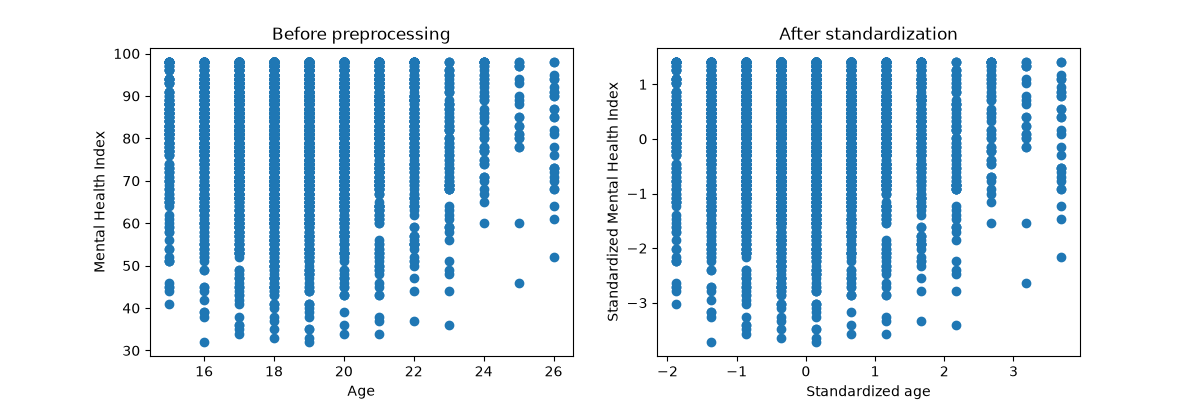
\includegraphics[width=\textwidth]{comparison.png}
  \caption{Idade e índice de saúde mental antes e depois da padronização}
  \label{fig:comparacao}
  \fonte{Elaborado pelos autores (2026).}
\end{figure}

\FloatBarrier

A ordem executada por \texttt{python main.py}, na raiz do projeto, é a seguinte:

\begin{enumerate}
  \item Carregar \path{data/raw/dataset.csv}.
  \item Selecionar as colunas numéricas.
  \item Preencher ausentes com a média truncada por idade.
  \item Padronizar com \texttt{StandardScaler}.
  \item Salvar a comparação de \texttt{Age} e \texttt{Mental\_Health\_Index}.
\end{enumerate}

\section{Código utilizado}

As listagens abaixo são os arquivos executados por \texttt{python main.py}, na ordem da chamada. O texto é o do repositório, sem alteração.

\subsection{Fluxo de execução}

Arquivo \texttt{main.py}.

\lstinputlisting{../../main.py}

\subsection{Leitura}

Arquivo \texttt{src/data/}\allowbreak\texttt{load\_data.py}.

\lstinputlisting{../../src/data/load_data.py}

\subsection{Seleção e preenchimento}

Arquivo \texttt{src/preprocessing/}\allowbreak\texttt{clean\_data.py}.

\lstinputlisting{../../src/preprocessing/clean_data.py}

\subsection{Média truncada}

Arquivo \texttt{src/calculations/}\allowbreak\texttt{descriptive\_statistics.py}.

\lstinputlisting{../../src/calculations/descriptive_statistics.py}

\subsection{Padronização}

Arquivo \texttt{src/preprocessing/}\allowbreak\texttt{standardize\_data.py}.

\lstinputlisting{../../src/preprocessing/standardize_data.py}

\subsection{Figura de comparação}

Arquivo \texttt{src/visualization/}\allowbreak\texttt{charts.py}.

\lstinputlisting{../../src/visualization/charts.py}

\postextual

\begin{thebibliography}{9}
\bibitem{yadav2026}
YADAV, Harish. \textbf{Impact of Social Media on Life}. 2026. Conjunto de dados. Disponível em: \url{https://www.kaggle.com/datasets/harishyadav0506/impact-of-social-media-on-life}. Acesso em: 26 out. 2026.
\end{thebibliography}

\end{document}
